\documentclass[a4paper,11pt]{kth-mag}
\usepackage[T1]{fontenc}
\usepackage{textcomp}
\usepackage{hyperref}
\hypersetup{
    colorlinks,
    citecolor=black,
    filecolor=black,
    linkcolor=black,
    urlcolor=black
}

% decrease line spacing English
\usepackage{enumitem}
\setlist{noitemsep}
\setlist[itemize]{itemsep=5pt,topsep=0pt}
\setlist[enumerate]{itemsep=5pt,topsep=0pt}

% remove "Chapter X" and a separate line
\usepackage{titlesec}
\titleformat{\chapter}{\normalfont\huge\bfseries}{\thechapter.}{20pt}{\Huge}

\usepackage{amsmath}
\DeclareMathOperator*{\argmax}{argmax}
\DeclareMathOperator*{\argmin}{argmin}

\usepackage{mathtools}
\DeclarePairedDelimiterX{\infdivx}[2]{(}{)}{%
  #1\;\delimsize\|\;#2%
}
\newcommand{\infdiv}{D\infdivx}
\DeclarePairedDelimiter{\norm}{\lVert}{\rVert}

\usepackage{caption}
\usepackage{subcaption}

\usepackage{graphicx}
\usepackage{lmodern}
\usepackage[latin1]{inputenc}
\usepackage[swedish,english]{babel}
\usepackage{modifications}
\usepackage[]{nomencl}
\makenomenclature
    \title{
      Label-Efficient Multi-Objective Machine Learning
      \\for e-Commerce
    }
    \subtitle{
      Exploration of transfer, multi-OBJECTIVE and active learning
      \\ across shallow and deep neural network architectures
      \\ for e-commerce product classification.
    }
    \foreigntitle{}
    \author{Mattias Arro}
    \date{June 2018}
    \blurb{Master's Thesis at KTH Information and Communication Technology
    \\      MSc Data Science (EIT Digital track)
    \newline
    \\Academic Examiner: Magnus Boman
    \\Academic Supervisor: Jim Dowling
    \\Industrial Supervisor: Abubakrelsedik Karali
    }
    \trita{2018}
\usepackage{imakeidx}
\makeindex[options=-s thesis]

\begin{document}

\frontmatter

% \pagestyle{empty}

\removepagenumbers
\maketitle
\selectlanguage{english}

\begin{abstract}
\noindent
Neural networks are powerful and flexible models capable of highly accurate predictions, transfer and multi-objective learning.
One of their biggest downsides is the amount of labelled data needed to train deep neural networks.
This work looks at three ways to tackle this label complexity problem: unsupervised and semi-supervised learning, transfer learning and active learning.
The former is described theoretically, and the usefulness of the latter two is evaluated through a series of experiments.
\\

\noindent
\textbf{Keywords:} machine learning, deep learning, neural networks, transfer learning, active learning, multi-objective learning, data-efficient learning, label-efficient learning, data engineering

\end{abstract}
\clearpage

% \begin{foreignabstract}{swedish}
% Denna fil ger ett avhandlingsskelett. Mer information om \LaTeX-mallen finns i dokumentationen till paketet.

% \end{foreignabstract}
% \clearpage

% \chapter*{Acknowledgment}
% ......
\noindent
London, UK, \today \\
\textit{Mattias Arro}


% \clearpage
\tableofcontents*

\mainmatter

\listoffigures

\newpage
% Example abreviations
\renewcommand{\nomname}{Abbreviations \& Definitions}

\nomenclature{rule-based}{labels and training objective produced by a deterministic keyword-matching system (1 ... n categories per product)}
\nomenclature{exclusive}{labels and training objective created by people applying manual labels (1 category per product)}
\nomenclature{exclusivised}{rule-based labels that have been converted toe exclusive by picking a random label of an exclusive category}
\nomenclature{embedding}{a multi-dimensional dense vector output by a neural network or learned through some other SGD process}
\nomenclature{ImageNet}{a large computer vision dataset and challenge}
\nomenclature{CIFAR10}{a computer vision challenge}
\nomenclature{MNIST}{a computer vision challenge consisting of hand-written digits}

\nomenclature{ML}{Machine Learning}
\nomenclature{NLP}{Natural Language Processing}
\nomenclature{BoW}{Bag of Words}
\nomenclature{BonG}{Bag of n-grams}
\nomenclature{TF-IDF}{term frequency - inverse document frequency}

\nomenclature{NN}{Neural Network}
\nomenclature{CNN}{Convolutional Neural Network}
\nomenclature{RNN}{Recurrent Neural Network}
\nomenclature{LSTM}{Long Short Term Memory}
\nomenclature{GRU}{Gated Recurrent Units}
\nomenclature{SGD}{Stochastic Gradient Descent}

\nomenclature{AE}{Autoencoder}
\nomenclature{VAE}{Variational Autoencoder}
\nomenclature{GAN}{Generative Adversarial Networks}
\nomenclature{WGAN}{Wasserstein Generative Adversarial Networks}
\nomenclature{CT-GAN}{a variant of WGAN}

\nomenclature{MF}{Matrix Factorisation}
\nomenclature{PCA}{Principal Component Analysis}

\nomenclature{KL divergence}{Kullback Leibler divergence}
\nomenclature{JS divergence}{Jensen Shannon divergence}

\nomenclature{ES}{ElasticSearch}
\nomenclature{GCP}{Google Cloud Platform}
\nomenclature{AF}{Airflow}
\nomenclature{TF}{TensorFlow}
\nomenclature{MLE}{GCP Machine Learning Engine}
\nomenclature{AutoML}{a GCP product for automatically training and tuning models}
\nomenclature{GCS}{Google Cloud Storage}
\nomenclature{UUID}{Universally Unique Identifier}

\printnomenclature



\pagenumbering{arabic}
\pagestyle{newchap}
\chapter{Introduction}

% \chapterprecishere{''Begin at the beginning'', the King said gravely,'' and go on till you come to the end: then stop.'' \par\raggedleft --- \textup{Lewis Carroll}, Alice in Wonderland}

 machine learning has become successful enough to be a recurring topic in popular science and mainstream media.
 


\section{Background}
\section{Problem}
\section{Research Questions}
\section{Purpose and Goal}
\section{Methodology}
\section{Evaluation}
\section{Work Environment}
\section{Deployment Environment}
\section{Ethics and Sustainability}
\section{Delimitations}
\section{Outline}

\chapter{Background}


\section{Input Representations}
\label{data_rep}

\subsection{Categorical Input}

The simplest option for representing categorical input is 1-hot encoding, where input has as many dimensions as there are distinct categorical values (vocabulary size); a single dimension is set to 1, with all other dimensions set to 0.
This is a straightforward representation: for a simple model such as logistic regression, we can clearly interpret the model parameters and see how the presence or absence of a given category increases or decreases the likelihood of a given output.
However, in cases where vocabulary sizes get  large, and the number of outputs (the number of units in the next layer in a deep network,  or the number of output units  in a shallow one) increases, this kind of encoding can really blow up the number of parameters of the model.
 this has many negative consequences: more memory, more required train data - curse of dimensionality

An alternative is to use  random embeddings:  dense, low-dimensional representations of a high-dimensional vectors.
It has been shown in compressed sensing literature that if a high-dimensional signal in effect lies on a low-dimensional manifold, then the original signal can be reconstructed from a small number of linear measurements \cite{compressive_sensing2}.
This has a useful implication for machine learning: categorical variables with large vocabularies of size \textit{d}  can be  represented with  random embedding vectors of size $M = \log(d)$.
This because it is possible to reconstruct any d-dimensional k-sparse signal using at most $k  log{\frac{d}{k}}$ dimensional vectors \cite{compressive_sensing1}, and 1-hot vectors are 1-sparse (only one dimension is nonzero).

An intuitive example is given in \cite{compressive_sensing3} about natural images: a 1-million-pixel image could have roughly 20,000 edges\footnote{technically: wavelet coefficients with a significant power, which roughly corresponds to a superimposition of edges}, i.e. it lies in a roughly 20,000-dimensional manifold from which the original image can be constructed with little loss in quality.
The 1-million-dimensional image could be projected into a M-dimensional space ``by taking M measurements of the image, where each measurement consists of a weighted sum of all the pixel intensities, and allowing the weights themselves to be chosen randomly (for example, drawn independently from a Gaussian distribution)''\cite{compressive_sensing3}.
The projection these random because the weights for the sum of pixel intensities are chosen randomly.
Why the projections need to be random is motivated by another intuitive example:  when light is shined on a 3-dimensional wireframe, its shadow is a 2-dimensional projection of it.
The projection could lose some important information about the regional object if the direction of the light source is chosen poorly,  however random directions are likely to result in projections where every link of the wire will have a corresponding nonzero length of shadow.

\subsection{Text Input}

The simplest way to represent  text is bag words (\textbf{BoW}),  which  is simply the histogram of word occurrences  in the text.
BoW  representations give equal weight to each of the words in the text, and the model has to learn the relative importance of each of these.
A commonly used representation in information retrieval (IR) is \textbf{TF-IDF},  which stands for ``term frequency -  inverse document frequency''.
TF-IDF  multiplies the term frequency (number of times the word occurred in the text) with its inverse document frequency ( the inverse of how often a occurs in all documents).
This has the effect of giving lower scores for common words, and higher scores for words which appear often in a document but not too frequently in the whole corpus.
Another common representation is bag of n-grams (\textbf{BonG}), which  is a histogram of character n-grams.

The above representations are sparse: there are vector representations grow linearly with the vocabulary size.
Text can also be  represented as a sequence of \textbf{word embeddings}.
Words and betting can either be random vectors or representations  learned with word cooccurrence algorithms such as word2vec \cite{} and GloVe \cite{};  these representations can remain fixed throughout the learning procedure, or updated as part of the stochastic gradient descent (SGD) when applicable.
A simple yet surprisingly powerful way to represent text is to average the word embedding contained in it \cite{}.
The  average could also be weighted by the TF-IDF score of each word\footnote{the author is unaware whether this has been tried before, but it seems a promising approach}.

More complex methods use recurrent neural networks (RNNs) to combine a sequence of word embeddings  into a \textbf{fixed length vector},  which are described in more detail in section \ref{rnn}.
These kinds of models are good at  disambiguating the potentially many meanings a word might have.
Exactly what gets persisted in the final  vector representation of text depends on how the model is trained - two RNNs  trained on different tasks (such as sentiment analysis and named entity recognition)  would need to store different information in its hidden state to successfully  perform their relevant tasks,  hence the encoding for the same sentence would be different for either model.
Still, an RNN  that is trained on one task could provide useful features for another.
Encoding text as fixed length vectors using RNNs has been interpreted as compressed sensing \cite{compressed_sensing_rnn}, with such vectors being ``provably at least as powerful on classification tasks, up to small error, as a linear classifier over BonG vectors''.

\subsection{Image Input}

Images can be represented as dense 3-dimensional tensor.
A 28x28 RGB image could be represented as a tensor with shape [28, 28, 3],  with the final dimension corresponding to the green, red, and blue intensity values at a given x/y coordinate.
These intensities  are usually in the range 0 ... 255, but are normalised before input to machine learning model.
Similarly to RNNs  encoding a sequence of words to a vector, 2D convolutional neural networks (2D CNNs)  can be used to extract dense feature vectors from raw images (image embedding),  further discussed in section \ref{image_models}.

\section{Models Considered}
\label{models_considered}

The following sections describes a selection of models that could be used for our classification task.
This is by no means an exhaustive list, nor is it a selection that is expected to have the highest predictive performance individually.
These models will later become part of an ensemble, where diversity matters much more than the performance of any individual model.
Engineering  considerations and time constraints also influence the selection of models: we did not want to spend time implementing models from scratch, or to use many frameworks for training models.
TensorFlow  is a widely used machine learning library with a good selection of open source models, in particular a selection of pre-trained models for computer vision and NLP, and has arguably the most mature deployment ecosystem.
Therefore models that did not have an open source TensorFlow implementation were automatically excluded.

Section \ref{general_models} describes models that can take categorical and text inputs, section \ref{text_models} looks at some neural models that take only text inputs, and section \ref{image_models} describes 2D CNNs that can classify or extract features from images.
In all cases the models are described in terms of how they could be used for solving the problem of multi-label classification.

\subsection{General Models}
\label{general_models}



\subsubsection{Logistic Regression}

Logistic regression is a linear, discriminative classifier that is often the baseline model of choice, since it is both interpretable and efficient to train.
There are methods that take time linear in the number of non-zeros in the dataset, which is the smallest amount possible, and it can be made to handle non-linear decision boundaries by using kernels \cite{murphy}.
Our case is the binomial logistic regression, with a separate logistic regression model for each output class.
This is shown formally in eq  \ref{logistic}, where where \textit{x} and \textit{w} correspond to the input and weight vectors, respectively.
We follow the notational trick where the first element of \textit{x} is always 1, and the first element of \textit{w} corresponds to the bias term.
The loss function of this model as well as how it is optimised is described in section \ref{loss}.

\begin{equation}
\label{logistic}
p(y|x,w)=\mathrm{Ber}(y|\mathrm{sigm}(w^Tx))
\end{equation}

\subsubsection{Feedforward Neural Network}

Feedforward neural networks (also called deep feedforward networks, multi-layer perceptrons) have been described as function approximator, whose goal is to approximate some functions $f^*$ \cite{dlb}.
We expect some familiarity with neural networks from the reader; for an excellent overview of the various use cases and models of deep learning, refer to.
In our case, the input is some representation of categorical and text input: sparse BoW or TF-IDF of text, 1-hot encoded or random embedding vectors of categorical variables, or embedding is extracted from text or images using pre-trained recurrent or convolution on neural networks.
The hidden layers of our network are homogenous: they use the same activation function (ReLu, sigmoid, or tanh) and have the same number of units;  activation functions and the number of units in hidden layers are determined through hyperparameter tuning.
The output layer uses sigmoid activation function  and has the same number of units as there are classes.

\subsubsection{Wide \& Deep}



\subsubsection{Loss Function and Optimizers}
\label{loss}

Logistic regression and neural networks are optimised with some variant of gradient descent.
For our task the loss function binary cross-entropy between the training data and the model distribution, with the loss value averaged across all classes.
This is given in eq. \ref{xentropy}, where $\theta$ corresponds to the model parameters such as the weights and biases of the model, $C$ corresponds to the number of classes, and $P(c=1|x, \theta)$ gives the predicted probability that the item belongs to class $c$ given the feature vector $x$.

\begin{align}
  \label{xentropy}
  NLL(\theta) &= \sum\limits_{c=1}^C \sum\limits_{i=1}^N\left[c_i\log P(c=1|x, \theta) + (1-c_i)\log(P(c=0|x, \theta) )\right]
\end{align}

We are minimising the negative log likelihood (NLL) rather than maximising the product of likelihoods.
Multiplying large numbers of probabilities could result in numerical underflow and rounding errors, therefore it is pragmatic to work with sums of log probabilities instead.
The Adam \cite{adam} optimiser works very well with default hyperparameters, and is therefore used for all stochastic gradient descent updates.

\subsection{Text Models}
\label{text_models}

\subsubsection{1D Convolutional Neural Networks}

A simple convolutional architecture for text classification is described in \cite{1dcnn}.
Pre-trained $k$-dimensional word vectors are concatenated to represent a sentence, and a filter is $w \in R^{hk}$ is applied to a window of $h$ words at each possible window of words in a sentence; this gives a single variable-length feature vector representing the sentence.
Several such filters are learned (each with potentially a different width $h$), and max-over-time pooling is applied to these feature maps; this gives a vector of the highest activations from each filter, which is then passed to a fully-connected softmax layer for final classification (in the case of multi-class classification).
For multi-label classification, the final layer would be a fully-connected layer of sigmoid activations.

This simple architecture should be able to predict output classes reasonably.
Each filter can indicate the presence of a a sequence of $h$ words; max-pooling discards information about where exactly in the text it appeared, and ensures the output is of a fixed length.
The same filter $w$ is used across all possible word windows in the sentence, which can be seen as a form of parameter sharing (and as an infinitely strong prior over the parameters of the model \cite{dlb}), and enables processing variable-length sequences.
The relatively small number of shared parameters requires less training data than an equivalent fully-connected architecture.
Using pre-trained word embeddings further simplifies the task, as these already carry some information about the meaning or syntactic role of words.

More sophisticated architectures can be built using 1D CNNs, although not used in our experiments.
Most notably, several layers of convolutions (each optionally followed by pooling) can be stacked, where the following layer works on the feature maps output by the previous layer.
The model described above uses a stride and dilation of 1, but multi-layer architectures where the higher layers have use exponentially increasing dilation are able to expand the receptive field of the model, and as a result aggregate ``contextual information from multiple scales'' \cite{dilated}.
Dilated convolutions were beneficial for semantic segmentation of images with 2D CNNs, but this increased receptive field has been useful for sequence-to-sequence models in NLP \cite{dilated_decoder}.

\subsubsection{Recurrent Neural Networks}
\label{rnn}

Recurrent neural networks (RNNs) are a family of models for processing sequential data.
The sequence of inputs $x^{(1)} \dots x^{(t)}$ in our case are vectors of word embeddings, but there are other options for input representations (e.g. sequence of 1-hot encoded tokens, or vectors representing a multivariate time series at a given time step $t$).
Vanilla RNNs maintain a hidden state vector $h$ which contains some information about the sequence it has seen so far, and is calculated from the input at the current time step $t$, and the previous hidden state:

\begin{equation}
  h^{(t)} = f(h^{(t-1)},x^{(t)})
\end{equation}

Vanilla RNNs suffer from the vanishing and exploding gradient problem in long sequences and are notoriously difficult to train.
Probably the most widely used variant, the long short-term memory networks (LSTM) \cite{lstm} overcome this limitation by augmenting the network with a memory cell $c$; there is a learned gating mechanism that controls what part of (and the extent to which) the cell is forgotten, what gets persisted in the cell state, and what gets output at a given time step.
An intuitive overview of the gating mechanisms is given by \cite{colah} and \cite{vanishing} describes well how this helps mitigate vanishing gradients.
A simpler gating mechanism is offered by gated recurrent units (GRU) \cite{gru}, which has fewer parameters and works well on simpler tasks.

We are interested in using RNNs as text encoders, though they are often used for sequence to sequence modelling, or for predicting an output at each time step.
In the simplest case, the concatenation of the cell state $c$ and the hidden state $h$ at the last time step could be used as a representation of the sequence.

\subsection{Image Models}
\label{image_models}

2D CNNs are important historically - excellent results in computer vision revived interest and funding in deep learning - but also applicable to a wide range of problems.
Computer vision CNNs tend to be complex models with millions of parameters and dozens (or even hundreds) of layers.
It is very compute-intensive and time-consuming to search for new architectures, and the analysis of these is beyond the scope of this work.
Our goal is to use a CNN that has a reasonable performance without incurring unreasonable overhead.

The general architecture of a 2D CNN is as follows.
Patches of feature extractors are convolved over the x and y axis of the image; these are often small, e.g. 3x3x$c$ patches that span all the $c$ channels of the image ($c=3$ for RGB images), and convolution could be strided.
Former models used larger patch sizes, but stacking several smaller patches could achieve similar receptive fields while allowing for a larger number of non-linearities for the same number of parameters.
One or more layers of convolutions would be followed by a (often max) pooling layer.
Computer vision architectures tend to re-use the same sub-structure repeatedly: either the same kinds of convolutions followed by pooling, or the ``network in a network'' structure popularised by GoogLeNet \cite{googlenet}.
After a number of such repeated structures, there are normally a few fully-connected layers followed by a softmax layer.
In our case, the final layer would be a fully-connected layer of sigmoid activations.

Transfer learning has shown to be particularly useful in computer vision.
Successful computer vision models require a notoriously large training dataset, which would be hard to come by for every distinct computer vision task.
Instead, models are often initialised to the values of a model that has been trained on a large dataset such as Imagenet \cite{}, excluding only the last layer(s) of the model that has learned features that are specific to the original problem.
Representations learned at the lower layers are remarkably  universal and useful for other tasks.
Therefore pre-trained 2D CNNs can be used as feature extractors for various other tasks,  or the models could be fine-tuned to learn representations that are even more useful to the new task.

\subsection{Downstream Models}

\subsubsection{Item Similarity}
\label{bg_sim}

One of the most easily available item similarity measures for e-commerce companies is BM?\footnote{it is built into ElasticSearch, a popular NoSQL database with integration to Sphinx?, a full-text search engine}

\subsubsection{Recommender Systems}
\label{rec}

Several methods have been proposed that use dense embeddings learned by deep models that are used as part of a recommender system.
These are briefly described here to motivate our focus on models that obtain dense embeddings of products.

Models that deal exclusively with deep embeddings \cite{mvdl} require huge amounts of user-product feedback pairs, therefore the more interesting solutions are ones which work together with classical methods such as matrix factorisation (MF).
MF finds - purely from the implicit or explicit feedback users five to items - vectors of latent factors that represent each user's preferences and each item's ``qualities''; the inner product between a user's and item's latent factors gives a score of compatibility between the two.
Deep models can augment the item latent factors by injecting the embeddings learned for another task
The main difference in these methods is how the deep embeddings are merged into MF, and how the deep embeddings are obtained in the first place.
In \cite{cdl}, stacked denoising autoencoders are used for unsupervised feature learning of item data, while \cite{dl_mf} uses simply visual embeddings extracted from a 2D CNN pre-trained on ImageNet.

\section{Unsupervised and Semisupervised Learning}
\label{unsup}

This section explores ways in which unsupervised and semi-supervised learning can learn good feature representations and improve sample complexity.
Generic semi-supervised methods such as self-training are not considered, as one of our goals is to learn good representations, but also because these methods can reinforce poor predictions or do not make full use of all available unlabelled data.

Some generic methods can still improve the representations learned by our models when applied to models that learn deep embeddings in order to make predictions.
Entropy minimisation \cite{entropy_min} can be incorporated into models trained with SGD to encourage confident predictions of each class; this encourages the deep model to learn predictions that are strong predictors of some class and avoid producing features that produce mixed predictions.
More complex but very performant approach is Mean Teacher \cite{mean_teacher}. A student that gets a harder task (such as predicting from a noisy/adversarial example), and a teacher that gets an easier task (i.e. the teacher model is an ensemble, which is more accurate).
The student is trained on the prediction of the teacher; the teacher's parameters are an exponential moving average of the student's, updated after each minibatch.
The teacher's predictions are higher-quality than the student's (and can be applied on unlabelled data), while the student tries to continuously learn to learn a predictor that is robust to noisy and adversarial examples.

\subsection{Autoencoders \& Variational Autoencoders}

Deep autoencoders (AEs) can be used to learn low-dimensional representations of inputs.
Many variants exist,  but  the general pattern is to have an ``hourglass-structured'' neural network where the first half of the model shrinks the input, and the second half of the network reconstructs the original input.
Activations in the middle layer correspond to a dense embedding of the sample;  the shrinking layers need to  throw away some of the detail in the input, yet persists enough for the expanding layers to be able to reconstruct the original input with some fidelity.
The embedding contains information that is mostly unique to the data point, while the parameters of the encoding and decoding layers ensure that the reconstructed input is realistic.
It is common to add noise (Gaussian, dropout) to the input or the intermediate layers to increase resilience to noisy inputs and to prevent the autoencoder simply memorising each data point.

If the bottleneck layer is unconstrained, it will use a wide range of values to represent different inputs.
We would like embedding for similar inputs to also be similar, which is not always the case for ordinary autoencoders.
Variational autoencoders (VAEs) impose a prior distribution on the values of the embedding, often a multivariate Gaussian distribution with a diagonal covariance matrix, and the model is regularised during training to respect this prior.
The model is optimised to minimise the reconstruction loss and KL divergence between the model's distribution $z$ and the prior on it, which can be computed just from $\mu$ and $\sigma$ if the prior is a isotropic standard normal.
Enforcing the prior also means that the embeddings $z$ will occupy a smooth, contiguous space, which allows us to draw samples from the prior $\epsilon \sim \mathcal{N}(0, 1)\,$ and use that as the input to the decoder - this gives us a generative model, which would not be possible with ordinary autoencoders.
The output of the VAE is also probabilistic: e.g. for images, the output for a pixel would be a Gaussian distribution, which is sampled the same way as the Gaussians for $z$.

The VAEs described here are probabilistic models parameterised by neural networks for approximating the true posterior $p(z|x)$, since the exact posterior is intractable.
In practice, VAEs add an extra loss term (KL divergence) to AEs, and additional step to determining the embedding $z$.
There are two separate neural network layers from the bottleneck layer of the AE:  one for determining $\mu$ (the vector of means of the multivariate Gaussian), and one for determining $\sigma$ (the vector of standard deviations of the multivariate gaussian).
Given $\mu$ and $\sigma$, we can sample the final item embedding $z \sim \mathcal{N}(\mu,\,\sigma^{2})\,$.
Note that sampling of $z$ is a discrete decision that would normally stop gradient from propagating past this step, but we can use the reparametrisation trick introduced by \cite{vae} that turns the discrete decision into a deterministic function of $z = \mu + \sigma\epsilon$, where $\epsilon \sim \mathcal{N}(0, 1)\,$ is a random auxiliary noise parameter.


\subsection{Conditional Variational Autoencoders}

It is easier for linear models to learn from embeddings extracted with AEs, and embeddings from VAEs make the classes even easier to separate.
These are unsupervised methods that do not take advantage of labels in the training data.
In the semisupervised approach introduced by \cite{semi_vae} there are two inference networks: a discriminative classifier that outputs a categorical distribution from the input $x$, and a class-conditional encoder that takes as input both $x$ and the 1-hot encoded categorical label $y$\footnote{class-conditional encoder means that the encoder is aware of the class of the data point, i.e. the output distribution $z$ is conditioned on the class $y$ in addition to the original input $x$}.
The model is trained on both labelled and unlabelled data.
For labelled examples, the $x$ and $y$ are given as input to the model, which embeds it in $z$ as described earlier, and reconstructs the original $x$.
The value of $y$ is unknown for unlabelled data points; therefore the model is run $|y|$ times, encoding and decoding the data point conditioned on each possible class $i$; loss from these runs is averaged, weighted by the discriminator's estimate of the sample belonging to class $i$.
This approach is acceptable for small numbers of classes, but is impractical for many multi-class problems.
A solution uses the reparametrisation trick mentioned above: rather than running the procedure once per class, we take a Gumbel-softmax \cite{gumbel} to get a discrete estimate of $y$ that is still differentiable.

Such class-conditional VAEs can be used in any situation where unlabelled data is abundant but labels are scarce.
The discriminator's loss is optimised as part of the VAE's loss function, which means adding more unlabelled data can improve the accuracy of the discriminator.
The approach was developed and tested on the MNIST dataset, which consists of 28x28 grayscale images - a very simple dataset by today's standards.
Some reports have emerged that fail to reproduce this success on more complex datasets such as CIFAR-10, being outperformed even by PCA \cite{vae_bad}.

One related approach is offered by \cite{towards}, where a class-conditional VAE is used to generate synthetic data for a discriminator network, which has reportedly a higher accuracy in semisupervised setting than the approach described just above.
They use it for conditional text generation, but this approach of using the class-conditional VAE to synthesise training data to train a discriminator is applicable to any input modality.
In fact the general approach to ``dreaming up'' new training samples in the \textit{sleep phase} and training the classifier in the \textit{wake phase} was introduced already in \cite{wake_sleep}.
The current author has implemented this model and open sourced it\footnote{https://github.com/mattiasarro/seq2seq-cvae-tensorflow}.

\subsection{Generative Adversarial Networks}

Generative adversarial networks (GANs) are an interesting approach capable of synthesising realistic data, but also useful for learning good representations of data.
GANs have been most successful for image synthesis, but are in fact applicable to any kind of input data including text \cite{} and even mixed data types such as user profiles \cite{}.
In the GAN setting, there are two networks: a generator that tries to produce realistic synthetic samples, and a discriminator whose goal is to distinguish between synthetic and actual samples.
% The networks are trained as a min-max optimisation problem where the generator is optimised to ``fool'' the discriminator by producing samples that appear to come from the true distribution, and the discriminator is optimised to  determine which samples are synthetic.
Given that the training is stable enough, both the generator's and the discriminator's performance improves with time, resulting in more realistic synthetic samples, as opposed to the relative blurry images produced by VAEs.
The discriminator needs to learn good representations of the input to  accurately distinguish which samples come from the true distribution, and which samples are synthetic; as with many CNNs for computer vision, these representations can be useful for other tasks as well.
It has been shown that  linear models  from the embeddings learned by the discriminator outperform other unsupervised feature learning techniques such as k-means \cite{dcgan}.
At the time of writing, variants of Wasserian GANs (WGANs) achieve the best performance by improving training stability and preventing the generator from generating samples from a limited number of modes; this is achieved by minimising the Wasserian distance between the generator's and real data distributions, as opposed to minimising the JS divergence as was common before.
A performant variant of WGAN is CT-GAN, which adds a regularisation term to enforce a Lipschitz continuity condition over the manifold of the real data \cite{ctgan}.

\section{General Practices in Machine Learning}

We briefly list some techniques and approaches that could be used for many kinds of machine learning problems.
Some of these will be used in our experiments, yet some may not be pragmatic due to long train times and time constraints.

Bootstrap sampling, where data points are sampled from training data with replacement, can be used to repeatedly train the same model, and to observe the variance of its predictions.
Bumping can be used to train several models (of the same family) on bootstrap samples to move around in the model space, and will pick the model that best fits the training data.
This helps it explore a wider selection of models, but given that the original training data often also included as one of the bootstrap samples, this method  can still pick the model original model if it happens to have the best accuracy.

There are some versatile methods that can help regularise a neural network (deep or shallow), or to speed up convergence by improving  gradient updates.
L2  regularisation should always be used to decrease moral complexity and impose prior on the model parameters, which  implies that very high and very low values are unlikely.
Dropout can mitigate overfitting by preventing neurons from co-adapting, encouraging each to learn representations that are useful independently \cite{dropout}; this has been interpreted as training and exponential (in the number of parameters) number of models and averaging their predictions.

gradient clipping
layer norm
Batch normalisation is known to stabilise training and hence speed up convergence  by normalising each input to have unit variance and zero mean \cite{batch_norm}.

\section{Combining Models}
\label{bg_ensembling}

This section  introduces common ensembling methods.
Some of these (bagging, boosting)  are expected to consist of weak learners or models from the same model family, while others (committee methods, BIC, stacked generalisation) or more appropriate for ensembles of strong models.

Bootstrap aggregation (a.k.a bagging)   draws several bootstrap samples  from the training data,  trains are separate model per bootstrap sample,  and averages the predictions of these individual models.  This reduces the variance of predictions without increasing its bias and generally leads to  more accurate predictors \cite{bagging}.
Boosting is another common meta-algorithm that iteratively trains an ensemble of weak models, such that the data points that incurred a higher error on the previous ensemble are weighted more heavily, and each new weak model is added to the ensemble with a weight proportional to the weak learners accuracy.
A common boosting algorithm is AdaBoost \cite{adaboost}.

We are interested in ways of combining models that are separately trained and combined into a single predictor.
Simple solutions are voting or (weighted) averaging, where the weights can be found with k-fold cross-validation.
A more appealing approach is stacked generalisation, where a meta-learner is trained on the outputs of the individual models.
This meta-learner could be a relatively simple model, such as logistic regression or a decision tree, and the results of the meta-learner could be therefore quite interpretable.

One orthogonal approach to combining models is joint training of model components.
All models described here are trained using stochastic gradient descent, so in principle it would be possible to learn the parameters of all components (1D CNN, 2D CNN, RNN, DNN, logistic regression) as part of a single optimisation loop.
This would be an engineering challenge due to the different ways these model require their input to be represented and the large size of the model, and optimisation would surely be difficult.
In our case this would be clearly an overkill, but it would be an interesting research problem to examine whether joint training has advantages over ensembling in cases where we have different views of the data (in terms of considering different input dimensions or processing the inputs differently).
As mentioned in the Wide \& Deep paper \cite{wide_deep}, the wide component of the model has to just handle cases where the deep component falls short, and can therefore be simpler than it would need to be in an ensemble; analogously, jointly training different kinds of models neural networks would allow each component to be simpler.

One of the motivations for picking mostly deep neural networks as our ensemble components was their transfer learning capability: they all produce a dense feature vector (embedding) from which separate logistic regressions predict the class.
While it is useful to have separate embeddings for images, text and categorical variables, we would also like to have a compound embedding of each product.
A simple concatenation of all individual embeddings could be a useful (albeit a quite high-dimensional) representation to be used in downstream models.
Alternatively, we could use this concatenation as an input to a neural network, whose goal is to (1) reduce its dimensionality by removing redundant information and (2) predict the output classes from this compressed embedding.
The latter case could act as a kind of a (replacement for) the meta-learner, with the difference that it takes the penultimate (as opposed to the final) layer of each individual model as input.

% https://arxiv.org/abs/0911.0460
% TODO figure of meta-learner and embedding lear

\section{Active Learning}
\label{bg_al}

This section describes the main approaches to active learning;  details analysis is beyond the scope of this report.

The goal of active learning is to reduce the number of labels needed  to effectively train a machine learning model by  being selective about which data points to label.
The three general scenarios: membership query synthesis, stream-based selective sampling, and pool-based sampling \cite{al_survey}.
In the first scenario, the algorithm synthesises a datapoint and asks a label for it.
In stream-based selective sampling, and instance is sampled and  the model decides (while having access to the data point's features) whether to acquire a label or not.
In pool-based sampling, the model chooses which data point to label from the pool of all unlabelled samples.
Our use case is a version of pool-based sampling, where the algorithm picks out a batch of products to be labelled.
 up

\chapter{Method}


Several hypotheses were tested in this work.
Section \ref{data_pp} gives an overview of how input data was pre-processd.
Section \ref{architecture} describes the technical set up required for running all these experiments and deploying the model to production before delving into the specific experiments and their evaluation methods in sections [ref].

\hfill \break \noindent
The experiments were conducted in four distinct stages:

 \begin{itemize}
   \item Training a baseline model on the rule-based labels to get a sense of the difficulty of this problem. Since there is no fundamental difference in the way this model was  trained and evaluated compared to the other classifiers, this is described in section \ref{exp_models} with the others. After this step, employees of the client company labeled products that would become the ground truth dataset. The visual comparison feature was also subjectively evaluated at this stage.
   \item Training the independent classifiers to determine best performers (\ref{exp_models}).
   \item Training an ensemble of the independent classifiers (\ref{exp_ensembling}).
   \item Training up to 10 iterations of active learning on the strong predictor (\ref{exp_al}).
 \end{itemize}


 \section{Data Preprocessing}
 \label{data_pp}

There were around a dozen product features that affiliate networks provided.
Most of these features were either categorical or textual,  with just a single numerical feature (price).
Initially, the data was analysed using Dataprep, a Google Cloud Platform (GCP)  product for data wrangling, which at the time of use was in beta stage.
Dataprep  was used to process a sample of ~800 000 products;  it produced histograms of the values present in each feature column (see appendix \ref{dataprep}).

The histograms revealed that a lot of the input features were mostly empty, but also that many of the inputs that would naturally be considered categorical  had much more unique value in them then one might expect.
For example, each affiliate gives us the textual representation what they consider to be the category of the product,  but  rather than containing a small number of unique tokens, these contained all the full category paths along with the category delimiters, which  varied retailer by retailer (e.g.  it was common to see both ``Shoes > Sneakers'' and ``Shoes // Sneakers'').
Representing these as categorical variables would have blown up the input space, which would have  resulted in more parameters, each parameter having fewer examples to learn from.
Therefore, many such ``categorical''  were actually represented as text, which were tokenised and cleaned appropriately, allowing for better generalisation and smaller models.

There was a single numerical field: price.
This could have been min-max normalised to the range 0 ... 1, however there  was a small number of very high values that would have squash nearly all the other  prices.
Rather than  carefully considering  how to mitigate this,  the input dimension was dropped, because it is not likely to have much predictive value for product classification.
It would be trivial to bring this feature back, for example  when building a recommended system, where it would be much more useful.

A trickier question was how many distinct tokens or categorical values to keep per input column.
Keeping all of them would not have been sensible: there were still large numbers of tokens that appeared only once, often because there were some unwanted formatting characters, misspellings, or incorrect punctuation that caused a token to be considered a separate entity.
There was a single configuration file that dictated which models used which features as input, whether those inputs were represented as textual, categorical, or dense values;  it also determined  the maximum number of unique values/tokens,  and the dimensionality of the embedding.
This configuration file was read by Dataflow during pre-processing  and by TensorFlow during  inference and training, which made experimentation with  different types of models and input representations considerably easier.

Below is a list of input features with information about how they were represented; it also lists the dimensionality of embeddings  for the models which  encoded categorical variables as embedding.

\begin{itemize}[noitemsep]
  \item title - text - max 8000 unique tokens
  \item brand - categorical - max 5000 unique values - 10 embedding dimensions
  \item category - categorical - max 950 unique values - 6 embedding dimensions
  \item rawCategory - text - max 1000 unique tokens
  \item description - text - max 8000 unique tokens
  \item gender - categorical - take all unique tokens
  \item size - categorical - max 100 unique tokens
  \item image - dense vector of 2048 features extracted with a 2D CNN
\end{itemize}

\subsection{Category Structure}
\label{cat_tree}

At the time of writing, there were roughly 1000 categories defined in the client database.
Categories were structured in a way that is typical of  e-commerce:  categories can have  child categories, which in turn can have child categories, etc.
In our case, the typical depth of the tree structure was five, i.e. a leaf category often had four parents;  naturally, the tree structure was not balanced, so many branches ended at depth three or four.

This structure has to be taken into account when labelling and  predicting categories for unseen products.
When a product is labelled to belong to a  lower level category,  it should also be labelled to belong to all of its ancestor categories. This does not work the other way around, though:  if a product is labelled not to be a Trainer (lower level category),  this does not imply it is not a Shoe (ancestor category).
Similarly, when the model predicts that a product belongs to and  lower level category, it is considered that it also predicted the product to belong to all of its  ancestor categories;  again, negative predictions at lower levels do not  overwrite positive predictions at high levels.

Note that the decision to consider each of the outputs as an independent binary variable in favour of mutually exclusive categories may later change.
There are some benefits to this: in some cases categories are inherently ambiguous, and allowing overlapping categories would enable us to use the same model to learn other attributes of products which might be more subjective.
For example, we might be able to train a model to distinguish certain styles within a category, which would not have clear boundaries.
Predicting binary independent outputs means that when a product is given a label (that it belongs to a category X),  this label does not immediately  exclude it from other categories;  with mutually exclusive categories labelling a product  would immediately determine whether or not it belongs to any of the categories.

\subsection{Class and Label Imbalance}
\label{label_imbalance}

The labels provided by the rule-based system are only positive:  some products are labelled to belong to a given category, but many products that ought to belong to a category are not labelled  accordingly -  but their label still appears to be negative.
This (which we call the label imbalance problem) only exacerbates the class imbalance problem (that most products do not belong to most categories).
As a result the model trained on rule-based labels will certainly underestimate the likelihood of any product belonging to any category.

Still, most positive labels provided by the rule-based system are correct, which means the model should assign higher likelihoods to products that should actually belong to the given class.
Our active learning strategy outlined in section \ref{exp_al} ensures that products around the decision boundary would receive a label - which during the initial rounds of active labelling would be overwhelmingly positive examples\footnote{this is confirmed by our experiments, described in section [ref]}.
The first rounds of active labelling should therefore counterbalance the underestimating nature of the pre-trained model; as the model starts to make more ``optimistic'' predictions, the products near the decision boundary should become a more balanced mix of positive and negative examples.

Class imbalance may or may not be an issue after label imbalance has been accounted for.
The worst case scenario is that our model continues to underestimate the likelihood of products belonging to classes, particularly if these are rare classes.
False negatives are not much of our problem in our setting.
There are millions of products that affiliate networks provide, and in any case we can show the average user a tiny fraction of those products, so it is okay if some are left out from some categories and their chance to be seen decreases.
Conversely, false positives will appear unprofessional and reduce user satisfaction.

% If label imbalance remains an issue, one might try to weight the loss function (eq \ref{original_loss}).
% The binary cross entropy loss function we use has two parts per class: the loss incurred for a false positive (FP) and false negative (FN) prediction.
% A weighted version (eq \ref{weighted_loss}) the loss function would wait the false-positive part of the loss function with the fraction of products that belong to that class, and the false negative part of the loss function with the fraction of products that do not belong to that class.
% We do not know how many products actually belong to a given class, and we would need to get this estimate through random sampling.
%
% \begin{align}
%   \label{original_loss} NLL(\theta) &= \sum\limits_{i=1}^N\left[FP + FN )\right] \\
%   \label{weighted_loss} NLLW(\theta) &= \sum\limits_{i=1}^N\left[P(y=1) FP + P(y=0) FN )\right] \\
%   FP &= y_i\log P(y=1|x, \theta) \\
%   FN &= (1-y_i)\log(P(y=0|x, \theta)
% \end{align}
%
% This weighting scheme is motivated by how imbalanced classes in multi-class classification can be handled.
% One option would be to oversample data points from the underrepresented class, but this would incur overhead in computation, and an equivalent method is to  weight the training example based on the class probability, so data points from underrepresented classes get a higher weight.
% As we have several independent output classes, the weighting would have to be done at the loss function level rather than per example.
% Note that the author could not find examples of the weighting scheme in literature, and is therefore not sure whether it is appropriate.

\section{System Architecture}
\label{architecture}

 The following technologies were used to build the system which had to interact with existing services  at the client company:

\begin{itemize}
  \item Apache Airflow (AF) - a Python framework for defining workflows of long-running tasks and dependencies between these tasks.
  \item TensorFlow (TF) - ML framework for Python, capable of defining many kinds of models as a computation graph, and executing this graph locally or in a distributed manner.
  \item ML Engine (MLE) - a GCP service for running TensorFlow models (training, hyperparameter tuning, inference).
  \item Apache Beam - a data processing engine akin akin to Apache Spark and Apache Flink.
  \item Dataflow - a GCP service for executing Apache Beam workloads.
  \item Tensorflow Transform - a Python library with a small set of operations for data preprocessing that can run inside a TensorFlow graph as well as an Apache Beam pipeline.
  \item Google Cloud Storage (GCS) - Google Cloud Platform (GCP) object storage similar to Amazon S3.
  \item ElasticSearch (ES) - a NoSQL database with powerful full-text search and querying capabilities.
  \item RabbitMQ - a message queue, used for transferring data among our microservices (using the Logstash adapter, that can read from and write to (among other things) ElasticSearch and RabbitMQ).
  \item Flask - a simple backend web framework for Python.
  \item Node.js - a JacaScript backend web framework.
  \item React.js - a JavaScript front-end framework for JavaScript.
  \item Redux - a framework for persisting user interface (UI) state and application data in single page applications.
  \item GraphQL - a query language for building flexible APIs
\end{itemize}

Figure \ref{arch_diagram} shows the how data is passed between the main services, and how services and technologies interact.

All product data is stored in ElasticSearch (ES): the rule-based labels, the predictions of the ML system, and evaluation metrics from various train runs.
ES is accessed from the public web application via GraphQL and the ML administration web UI (further referred to just as web UI\footnote{The web UI was initially built with Flask and React by the author as a quick way to get insight about the model, and then re-written as a more feature-rich version by an employee of the client company with Node.js, GraphQL, React and Redux.}).
Data is pulled into the ML pipelines by dumping the results of an ES query to a local file, which is uploaded to GCS.
Updates to the ES index are not done directly, since indexing the updated products is computationally expensive; instead, updates are put on a RabbitMQ queue, which is consumed by Logstash, which in turn updates products in ES at a rate that will not overburden the servers.

All ML training and prediction happens in a batch-oriented way, encapsulated as Airflow pipelines.
Each pipeline is a directed acyclic graph of tasks, where a task can be a shell command or Python function; a pipeline defines dependencies of task execution, which allows us co-ordinate a series of operations that could be executed locally (inside the Docker container running AF) or remotely (such as in a GCP service).
A typical pipeline dumps data locally, uploads it to GCS, schedules a Dataflow job to preprocess data, polls the Dataflow service until the Dataflow job is finished, schedules an ML engine job, polls the MLE service until it has completed, and runs an update process that reads the predictions and evaluation statistics from GCS and sends the updates to the RabbitMQ queue.
Reading updates and sending these to RabbitMQ is done in a parallelised manner (using multiprocessing), since the update process is bottlenecked due to network latency as well as computing the appropriate category path for each product (explained in \ref{cat_tree}).

\begin{figure}
  \hspace*{-0.2\textwidth}
  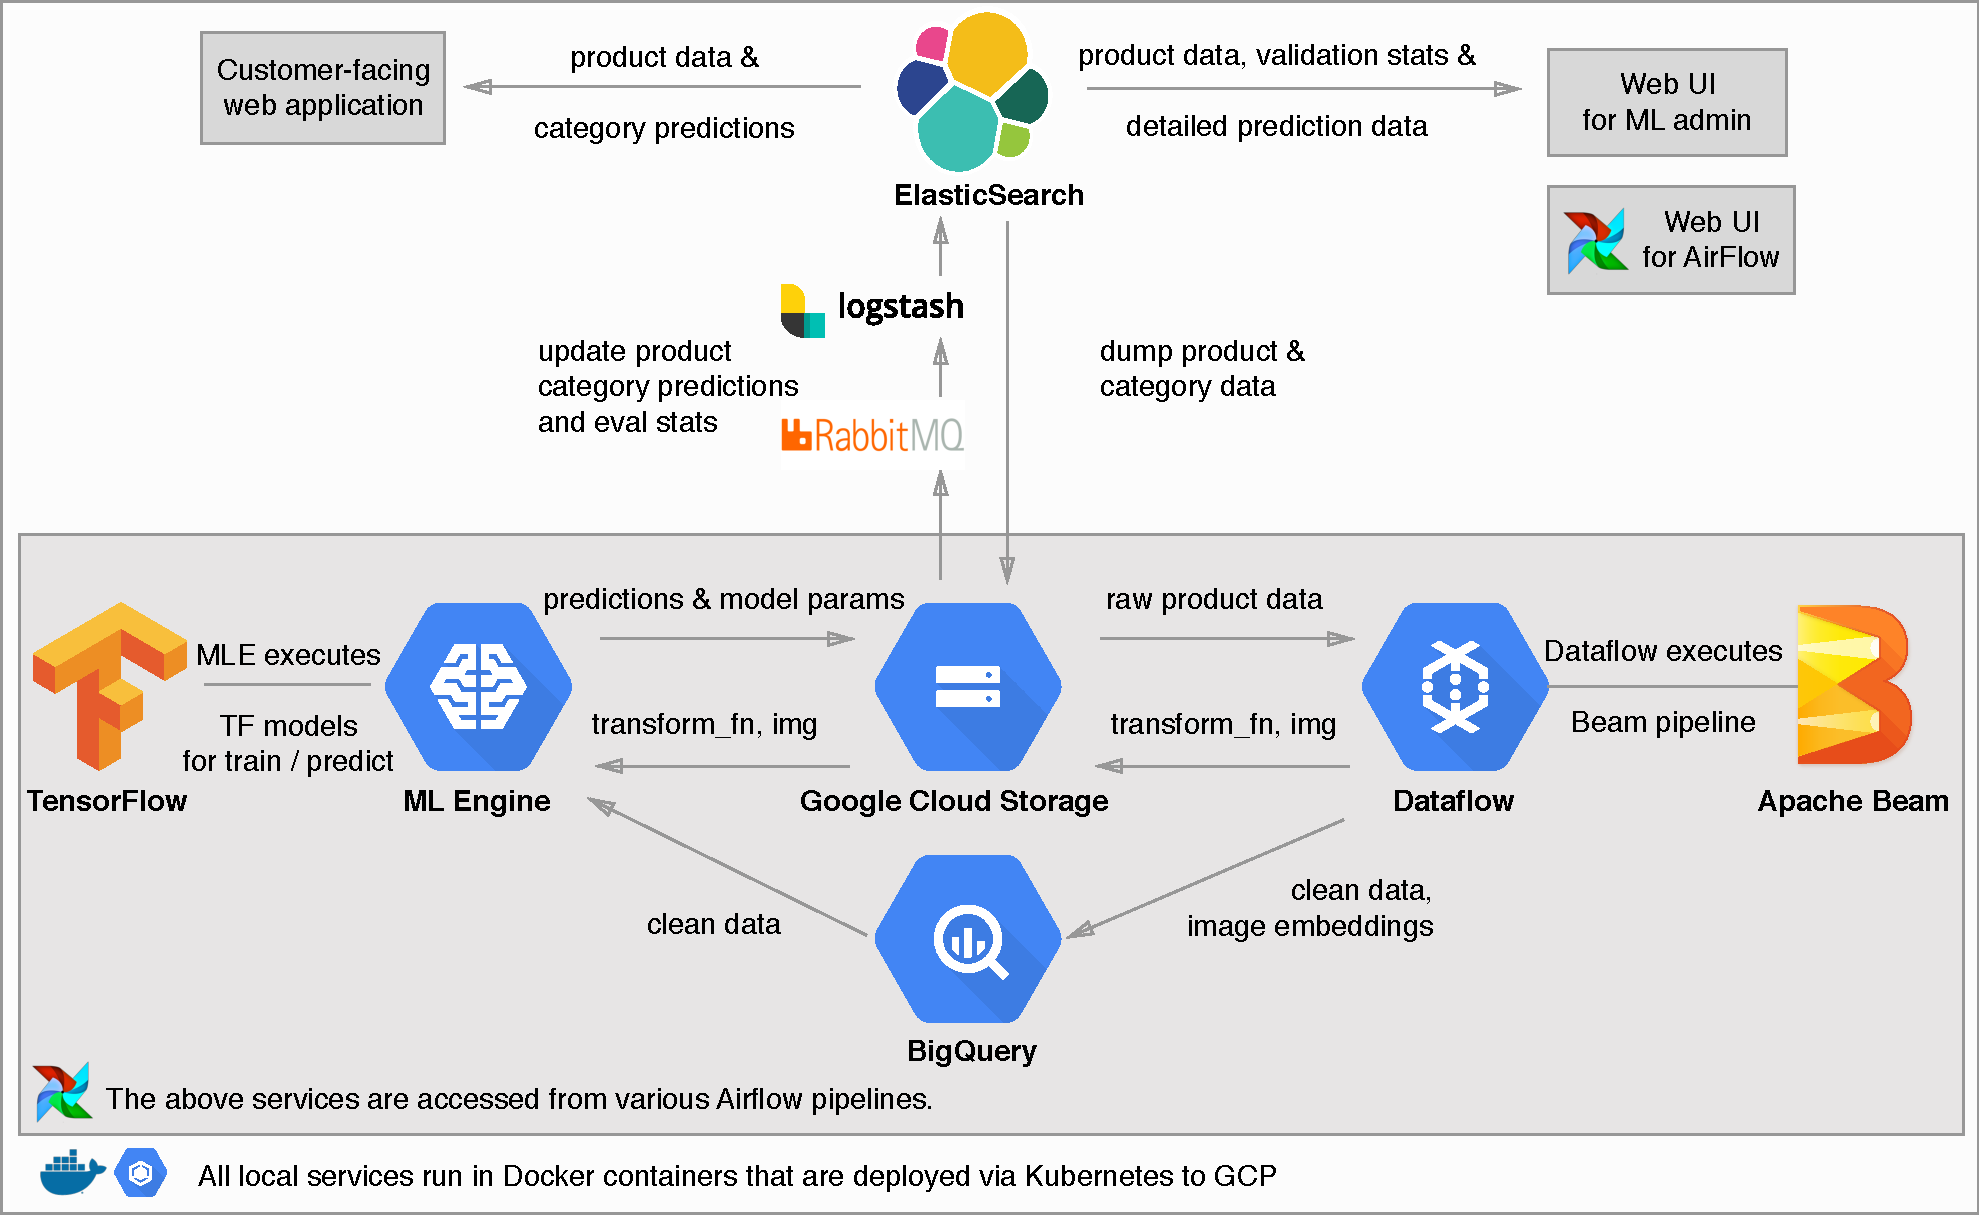
\includegraphics[width=1.4\textwidth]{diagrams/architecture}
  \caption{High-level system architecture of the ML pipeline}
  \label{arch_diagram}
\end{figure}

\subsection{Dataflow Pipelines}
There are two types of Dataflow pipelines: for preprocessing training data and for calculating product-product visual similarity. Omitting various details, dead-ends and workarounds that were needed due to technical limitations and prior system architecture choices\footnote{which were completely reasonable at the time, when the ML system was not a consideration}, the pipelines had the following tasks:

\subsubsection{Preprocessing}

This pipeline loads the products dumped from ES (as JSON) and preprocesses data according to a configuration file (see section \ref{data_pp}).
All fields are cleaned of obvious noise and superfluous whitespace.
Text and categorical fields are tokenised and mapped to integer indices, keeping only the top \textit{k} values and also computing TF-IDF scores for text fields.
This is handled by TensorFlow Transform, which persists this token-to-index mapping in a \textit{transform function} that is saved to GCS at the end of the pipeline.
The transform function is used by a TensorFlow model to convert raw text inputs to a  sparse inputs;
separate pre-processing run will generate a different transform function, with mostly the same tokens mapping to different indices, as the order in which they will be encountered will be different.

The pipeline is also responsible for downloading product images and using a pre-trained 2D CNN to extract a dense feature vector for each product from the penultimate layer of the CNN.

The clean data and image embeddings  are inserted into a new BigQuery table after each run\footnote{BigQuery is inefficient in updating existing records and limits the number of update per day}.
Note that the data is not inserted in its tokeniser form.
Storing tokeniser data would reduce the space it takes marginally, but keeping raw data makes the system easier to debug, and enables the option to do inference on raw data that is not tokenised (e.g. in a streaming banner, when we might not have access to the transform function).

\subsubsection{Visual Similarity}

% maybe bigquery is not the best choice

This Dataflow pipeline uses the data in BigQuery as input.
As explained in section \ref{exp_sim}, it needs to find the \textit{k=100} nearest neighbours of each product based on the cosine similarity of their image embeddings.
The product-product  similarities are computed within products that belong to same second level category,  therefore the pipeline only needs to extract  the categories previously predicted and image embedding from BigQuery.
The resulting predictions (top 100 product UUIDs per product, ordered by  similarity)  are saved to GCS.

\section{Experiments}

\subsection{Visual Similarity}
\label{exp_sim}

ann
tfidf-based

\subsection{Independent Models}
\label{exp_models}

\subsection{Ensembling}
\label{exp_ensembling}

\subsection{Active Learning}
\label{exp_al}


\section{Evaluation}
\label{evaluation}

At the beginning of running all these experiments, the dataset was divided into development and test set (90/10\%).
The development set was used for


 we can evaluate the performance of the model on three types of datasets:

\begin{itemize}
  \item the test or validation set as labelled by the rule-based system (referred to as ``rule-based test/validation set''),
  \item the ground truth dataset gathered  before running most experiments,
  \item
\end{itemize}

\chapter{Discussion}
\label{disc}

In this section we analyse the experiments that were described in the previous section.

\section{Visual Similarity}

Although this assessment is subjective, the results from the approximate nearest neighbour were strikingly good; this is the opinion of many people at the client company that saw a demo of it.
The model did not require fine-tuning, contrary to the initial hypothesis.
The biggest challenge here is to find a way to evaluate visual similarity performance; although there are various algorithms for tweaking similarity and evaluating it on a test set, creating such a dataset would have been prohibitively expensive.
Given that vanilla pre-trained CNNs produce good embeddings for visual similarity, it is sensible to focus one's efforts on the scalability and productionalisation aspect of this problem.
Still, two relatively easy directions could yet be explored: the model architecture and the layer from which embeddings are extracted.
Our model of choice was Inception V3, which had a good accuracy to memory footprint ratio - with respect to the original ImageNet challenge.
However it has been shown that models that are well tuned for a given classification task are not necessarily the best feature extractors; in fact, ResNets are currently the best at this \cite{img_feature_extract}.
The other decision of of using the penultimate layer of the CNN as a feature extractor is also a common one.
Often the transfer learning task is classification, for which the higher-level fully-connected layers would provide good high-level semantic features.
In our case, extracting features from the first fully-connected layer or even from the raw convolutional feature maps at a lower layer might have given us similarity that is highly sensitive to certain visual patterns and shapes - which could be deployed to certain categories where such sensitivity is required.

As already discussed, the tokenised versions of feature vectors had less spectacular results.
While appealing as a way to combine visual and textual similarity, there is not theoretical justification for this approach.
Note that the original paper \cite{vec_fulltext} extracted dense features from text, and only hypothetically proposed this approach to be applied on images.
Perhaps the inherent discrete nature of language (sentences, words, topics as opposed to a continuous 2D space)  makes it more amenable to such tokenisation.

\section{Individual Models \& Hyperparameters}

Choosing a relatively complex model such as Wide \& Deep as a baseline model can be criticised: a baseline should be simple and interpretable.
One of the justifications was the ability to turn some part of the model off, as removing all deep input columns would have resulted in a linear model and vice versa\footnote{Implementing separate model types (deep, linear, wide \& deep) turned out to be simpler.}.
The other intuition was drawn from models with skip connections such as ResNets \cite{resnet} and DenseNets \cite{densenet}.
The assumption was that linear models are relatively good at predicting the output, as the relevant word tokens would be present in the textual fields of many products; for a deep model to use this raw knowledge, it would need to learn an identity function from the input of the layer to the output, which can be a hard problem with some activation functions.
Therefore, a linear layer with the same input as the deep layer could be justified to simplify learning for such simple cases, though not necessarily as the first ``baseline''.
Overall Wide \& Deep performed very well, though it is hard to compare its PR AUC to the other models, which were trained and evaluated on twice the amount of data.
When its performance degraded once it was trained on a new dataset (that most likely had mixed up image embeddings of some products), its drawback became apparent: we had no clue which of the input features were most responsible for good or bad performance.

Training a large selection of deep and shallow models was a good way to get a sense of the capabilities of these models.
The performance of linear models was lower than expected, but this is probably not a fair comparison, as the models were trained on the same sets of hyperparameters that were at least in part chosen to be suitable for deep models.
In general the tools used (TensorFlow, Adam optimiser) may not be optimal for learning linear models, but considering the large difference of PR AUC between the two, there seem to be benefits to using deeper models.
Contrary to our hypothesis, deep models with 1-hot / k-hot inputs did outperform shallow ones, but the difference in performance decreased when the models received a bigger selection of input features.
This implies that deep models are indeed generalising better from a small set of inputs; for example, the deep model that received averaged word embeddings of the title continued to improve even at epoch 6, and received a remarkably better PR AUC score (0.93) than its linear counterpart (0.42, or 0.53 for linear with k-hot inputs).

The biggest problem in interpreting the PR AUC scores of the rule-based objective is that its labels were generated using a relatively simple automatic procedure which only considers text as its input.
Therefore a high PR AUC score shows us only how well the model was able to reproduce the behaviour of the rule-based system, but we are after good generalisation and consistent multi-objective performance.
Therefore good results from title-only models should be taken with a grain of salt.
We consider the classification problem to be a quite easy optimisation problem, however the power of more complex models might be better served when we are adding more training objectives (e.g. colour, style, conversion of products).

Some patterns emerge from training this selection of models.
For linear models, 1-hot and k-hot encoding always outperforms embedding inputs, which was contrary to our hypothesis.
Deep models pre-trained on other objectives are quite consistent in their generalisation, producing strikingly similar PR AUC and recall scores whether it takes the title, description or image as input.
Examining the true/false positives/negatives of individual classes reveals that these models are relatively good at predicting certain classes, yet fail to differentiate between more specific ones.

It would be interesting to compare the performance of these models with random forests and 1D CNNs; fine-tuning of pre-trained models would also be an interesting comparison, as would models trained on character n-gram representations or TF-IDF-weighted embeddings.
Our embedding models could further be improved by not limiting the number of unique tokens so aggressively; as embedding based models have shown to perform better than 1-hot encoding in deep models, we could expand the vocabulary sizes without increasing input dimensionality.

Hyperparameter tuning using Bayesian optimisation was not as successful as expected.
In the first round where the Wide \& Deep model was tuned, the final metric value was only marginally higher than PR AUC of manually chosen hyperparameters, yet the model complexity was far greater.
A simpler model with comparable accuracy is more likely to generalise better, therefore most of the following deep models used 4 layers.
In the second tuning round, the model failed to learn in any instance; this is probably because the large range supplied for the ``L2 scale'' parameter.
An examination of the individual models that were trained during tuning showed that L2 decay overpowered the training loss and resulted in a very strict model that nearly always predicted the negative class.
The rate weight decay scaling parameter was kept fixed at 0.0005 for future runs based on analogous values used in literature; there is also some evidence that one should specify a custom scheme of weighting the L2 loss with adaptive optimisers such as Adam \cite{fix_adam}.

Given that we were training models with high capacity, it would also be useful to know the variance of the outcome if the model is trained several times by doing k-fold cross-validation.
Due to the large dataset size and time limitation this was not tried formally, however these models were trained across dozens of different data pre-processing runs during which the train/validation split was different.
There was not much variability within even the high-capacity models, which often converged at a high AUC PR score.

\section{Multi-Objective Training}

Even though the rule-based objective gave good PR AUC scores, the model was not deployable as is, since it severely under-predicted all nontrivial categories.
As one might expect, training for multiple objectives has a higher variance in the gradients.
This was exacerbated by the limitations of the tf.data APIs, which did not enable to efficiently alternate between the training objectives precisely.
Probably the variability could be reduced if each batch had a consistent number of products from each objective.
For more thorough experimentation, one should probably fall back to manually feeding data batch-by-batch, as was the standard in earlier versions of TensorFlow.

Although Adam was a versatile optimiser across the different deep and shallow architectures for the rule-based objective, updates to the parameters of each top layer becomes less frequent in the multi-objective case.
As Adam learns to update less frequently updated variables more heavily, this is probably the cause of a wide range of issues described in section \ref{multiobj}.
Note that it is not formally confirmed that the peculiarities are caused by adaptive learning rates.
Experimenting with a simpler optimiser and outputting per-step statistics about how many data points from each objective ended up in each bach would help further understand the shape of the loss functions.
For example, currently the best guess to the peculiar shape of the rule-based training loss (blue line in figure \ref{pretrain}) in a multi-objective training setting is that the large jumps are caused by a large batch of data points from the exclusive objective which has had few updates in a while; the medium-variance periods that follow such jumps (e.g. steps 40k - 80k) also contain data from that objective; the gradually decreasing plateaus (e.g. steps 80k - 120k and 170k - 200k) are periods where the model is trained only on the rule-based objective, which is considerably more stable.

It is satisfying that a multi-objective training scheme outperforms a method trained on just exclusive labels.
Though the exclusivised objective at times exceeds multi-objective training in terms of accuracy, the latter is preferred due to its stability and predictability; also, this scheme will be useful once we add additional training objectives.
The 60\% on the exclusive objective is not ideal.
This is achieved with roughly 6000 manual labels, which is far from the millions of labels deep neural networks usually require.
Probably the biggest gains will come from re-organising the category tree further so that there are no ambiguous classes, and that all the ambiguous cases (e.g. ``Leather Jackets'') are handled as a combination of an exclusive class (``Jacket'') and independent feature detector (``Material: leather'').
The remaining gains will come from active labelling, which should find the uncertain cases, or by manually adding labels to categories with a high error rate.
An orthogonal approach is to train using the Wasserstein loss, which would be better at handling ambiguous and noisy labels; in this case, we might use the Wasserstein distance between the predicted and actual labels as the evaluation metric as well, as accuracy would still paint a pessimistic picture when in reality it is acceptable to classify into a semantically nearby class.
Different training regimes could still be tried to stabilise multi-objective learning, such as gradient clipping, layer and batch normalisation.

A separate question is how to phase out the old rule-based system that the client company wishes to replace.
As the rule-based system would stop producing labels, any new products would be unlabelled according to it.
This would happen more often than one might think due to the way the data import process happens.
The most likely solution is to create an interface for mass-labelling of products: present the labeller pages with hundreds of products that are predicted to belong to a category, and have them confirm the page or pick out incorrect predictions.
This way we create a large number of high-quality labels with relatively little effort.

\section{Active Learning}

Preliminary results indicate that uncertainty sampling is effective at identifying products that might lack a category or sufficient labels in the training data, but it tends to sample products that are very much alike.
Therefore this strategy may not be very well suited for such a ``batch-active'' learning scenario as was presented.
A workaround might be a series of smaller training rounds.
Identifying unseen categories is a useful feature, though an analysis of validation error might produce similar results.

\chapter{Conclusion}
\label{sum}

In this work we covered a large breadth of topics.
Neural networks and deep models have many useful qualities: their performance continues to improve with additional training data, they can be successfully used for transfer and multi-task learning, and they can synthesise realistic samples of their own.
In general, deep models based on embedding inputs outperform ones with sparse inputs, while linear models do well with 1-hot encoded inputs.
Transfer learning is remarkably useful, as our experiments with visual similarity show, though models trained from scratch on raw product data is still superior for fine-grained affiliate product classification.
While this work did not experiment with ensembling of models, we did look at joint training of models that individually performed reasonably well, and as was expected found that a combination of all these inputs outperforms any subset.

A big part of the time spent on this project involved building the technical architecture.
This was a non-trivial task given the large number of technologies, distributed components and dataset sizes involved.
This could serve as a blueprint for many projects that are planning to deploy to the GCP cloud.

Our experiments with multi-objective training ultimately produced the expected results, and the performance increase could be hopefully improved with more analysis of the high gradient variance during training.
Even though a good number of models were trained to optimise hyperparameters using Bayesian optimisation, the bulk of these were still picked based on intuition.
At the very least, such tuning reveals that at least for this problem the models are not too sensitive to hyperparameters.

The results from active learning are not yet conclusive, though the tentative conclusion is that uncertainty sampling should not be used too early when the model is not yet close to an optimal solution, as it might sample very similar data points.
Our experiments are still in progress, though, and a later evaluation might conclude something more positive.

Overall, the choice of tools and approaches was reasonable.
There are clearly more straightforward ways to do product classification, yet the complications introduced by transfer, multi-objective and active learning will most likely pay off when predicting much more difficult aspects, such as whether a product would sell well for a given audience or not - which has immense potential to increase profitability.


\renewcommand\bibname{References}
\bibliographystyle{plain}
\bibliography{extras/_bibliography}

\clearpage
\pagestyle{empty}
% \renewcommand*{\chapterpagestyle}{empty}
\chapter*{Declaration}




\vspace*{2cm}
\noindent
I hereby certify that I have written this thesis independently and have only used the specified sources and resources indicated in the bibliography.

\vspace{2cm}

\noindent
London, UK, \today

\vspace{3cm}

\hspace*{7cm}%
\dotfill\\
\hspace*{8.5cm}%
\textit{Mattias Arro}
\addcontentsline{toc}{chapter}{Declaration}


% \appendix
% \addappheadtotoc
% \chapter{Additional Background}

\section{Neural Models}

\subsection{1D Convolutional Neural Networks}
\label{1d_cnn_app}

A simple convolutional architecture for text classification is described in \cite{1dcnn}.
Pre-trained $k$-dimensional word vectors are concatenated to represent a sentence, and a filter is $w \in R^{hk}$ is applied to a window of $h$ words at each possible window of words in a sentence; this gives a single variable-length feature vector representing the sentence.
Several such filters are learned (each with potentially a different width $h$), and max-over-time pooling is applied to these feature maps; this gives a vector of the highest activations from each filter, which is then passed to a fully-connected softmax or sigmoid layer for final classification.

This simple architecture should be able to predict output classes reasonably.
Each filter can indicate the presence of a a sequence of $h$ words; max-pooling discards information about where exactly in the text it appeared, and ensures the output is of a fixed length.
The same filter $w$ is used across all possible word windows in the sentence, which can be seen as a form of parameter sharing (and as an infinitely strong prior over the parameters of the model \cite{dlb}), and enables processing variable-length sequences.
The relatively small number of shared parameters requires less training data than an equivalent fully-connected architecture.
Using pre-trained word embeddings further simplifies the task, as these already carry some information about the meaning or syntactic role of words.

More sophisticated architectures can be built using 1D CNNs, although not used in our experiments.
Most notably, several layers of convolutions and pooling can be stacked, where the following layer works on the feature maps output by the previous layer.
The model described above uses a stride and dilation of 1, but multi-layer architectures where the higher layers have use exponentially increasing dilation are able to expand the receptive field of the model, and as a result aggregate ``contextual information from multiple scales'' \cite{dilated}.
Dilated convolutions were beneficial for semantic segmentation of images with 2D CNNs; increased receptive field has also been benefitial in sequence-to-sequence NLP models \cite{dilated_decoder}.

\subsection{Recurrent Neural Networks}
\label{rnn_app}

Recurrent neural networks (RNNs) are a family of models for processing sequential data.
The sequence of inputs $x^{(1)} \dots x^{(t)}$ in our case are vectors of word embeddings, but there are other options for input representations (e.g. sequence of 1-hot encoded tokens, or vectors representing a multivariate time series at a given time step $t$).
Vanilla RNNs maintain a hidden state vector $h$ which contains some information about the sequence it has seen so far, and is calculated from the input at the current time step $t$, and the previous hidden state:

\begin{equation}
  h^{(t)} = f(h^{(t-1)},x^{(t)})
\end{equation}

Vanilla RNNs suffer from the vanishing and exploding gradient problem in long sequences and are notoriously difficult to train.
Probably the most widely used variant, the long short-term memory networks (LSTM) \cite{lstm} overcome this limitation by augmenting the network with a memory cell $c$; there is a learned gating mechanism that controls what part of (and the extent to which) the cell is forgotten, what gets persisted in the cell state, and what gets output at a given time step.
An intuitive overview of the gating mechanisms is given by \cite{colah} and \cite{vanishing} describes well how this helps mitigate vanishing gradients.
A simpler gating mechanism is offered by gated recurrent units (GRU) \cite{gru}, which has fewer parameters and works well on simpler tasks.

We are interested in using RNNs as text encoders, though they are often used for sequence to sequence modelling, or for predicting an output at each time step.
In the simplest case, the concatenation of the cell state $c$ and the hidden state $h$ at the last time step could be used as a representation of the sequence.

\section{Unsupervised and Semi-supervised Learning}
\label{unsup_appendix}

This section explores ways in which unsupervised and semi-supervised learning can learn good feature representations and improve label complexity.
Generic semi-supervised methods such as self-training are not considered, as one of our goals is to learn good representations, but also because these methods can reinforce poor predictions or do not make full use of all available unlabelled data.

Some generic methods can still improve the representations learned by our models when applied to models that learn deep embeddings in order to make predictions.
Entropy minimisation \cite{entropy_min} can be incorporated into models trained with SGD to encourage confident predictions of each class; this encourages the deep model to learn predictions that are strong predictors of some class and avoid producing features that produce mixed predictions.
More complex but very performant approach is Mean Teacher \cite{mean_teacher}. A student that gets a harder task (such as predicting from a noisy/adversarial example), and a teacher that gets an easier task (i.e. the teacher model is an ensemble, which is more accurate).
The student is trained on the prediction of the teacher; the teacher's parameters are an exponential moving average of the student's, updated after each minibatch.
The teacher's predictions are higher-quality than the student's (and can be applied on unlabelled data), while the student tries to continuously learn to learn a predictor that is robust to noisy and adversarial examples.

\subsection{Autoencoders \& Variational Autoencoders}

Deep autoencoders (AEs) can be used to learn low-dimensional representations of inputs.
Many variants exist,  but  the general pattern is to have an ``hourglass-structured'' neural network where the first half of the model shrinks the input, and the second half of the network reconstructs it.
Activations in the middle layer correspond to a dense embedding of the sample;  the shrinking layers need to  throw away some of the detail in the input, yet persists enough for the expanding layers to be able to reconstruct the original input with some fidelity.
The embedding contains information that is mostly unique to the data point, while the parameters of the encoding and decoding layers ensure that the reconstructed input is realistic.
It is common to add noise (Gaussian, dropout) to the input or the intermediate layers to increase resilience to noisy inputs and to prevent the autoencoder simply memorising each data point.

If the bottleneck layer is unconstrained, it will use a wide range of values to represent different inputs.
We would like embedding for similar inputs to also be similar, which is not always the case for ordinary autoencoders.
Variational autoencoders (VAEs) impose a prior distribution on the values of the embedding $z$, often a multivariate Gaussian distribution with a diagonal covariance matrix, and the model is regularised during training to respect this prior.
The model is optimised to minimise the reconstruction loss and KL divergence between the model's distribution of and the prior on it, which can be computed just from $\mu(z)$ and $\sigma(z)$ if the prior is a isotropic standard normal.
Enforcing the prior also means that the embeddings $z$ will occupy a smooth, contiguous space, which allows us to draw samples from the prior $\epsilon \sim \mathcal{N}(0, 1)\,$ and use that as the input to the decoder - this gives us a generative model, which would not be possible with ordinary autoencoders.
The output of the VAE is also probabilistic: e.g. for images, the output for a pixel would be a Gaussian distribution, which is sampled the same way as the Gaussians for $z$.

The VAEs described here are probabilistic models parameterised by neural networks for approximating the true posterior $p(z|x)$, since the exact posterior is intractable.
In practice, VAEs add an extra loss term (KL divergence) to AEs, and additional step to determining the embedding $z$.
There are two separate neural network layers from the bottleneck layer of the AE:  one for determining $\mu(z)$ (the vector of means of the multivariate Gaussian), and one for determining $\sigma(z)$ (the vector of standard deviations of the multivariate gaussian).
Given $\mu(z)$ and $\sigma(z)$, we can sample the final item embedding $z \sim \mathcal{N}(\mu,\,\sigma^{2})\,$.
Note that sampling of $z$ is a discrete decision that would normally stop gradient from propagating past this step, but we can use the reparametrisation trick introduced by \cite{vae} that turns the discrete decision into a deterministic function of $z = \mu + \sigma\epsilon$, where $\epsilon \sim \mathcal{N}(0, 1)\,$ is a random auxiliary noise parameter.


\subsection{Conditional Variational Autoencoders}
\label{gans}
It is easier for linear models to learn from embeddings extracted with AEs, and embeddings from VAEs make the classes even easier to separate.
These are unsupervised methods that do not take advantage of labels in the training data.
In the semi-supervised approach introduced by \cite{semi_vae} there are two inference networks: a discriminative classifier that outputs a categorical distribution from the input $x$, and a class-conditional encoder that takes as input both $x$ and the 1-hot encoded categorical label $y$\footnote{Class-conditional encoder means that the encoder is aware of the class of the data point, i.e. the output distribution $z$ is conditioned on the class $y$ in addition to the original input $x$.}.
The model is trained on both labelled and unlabelled data.
For labelled examples, the $x$ and $y$ are given as input to the model, which embeds it in $z$ as described earlier, and reconstructs the original $x$.
The value of $y$ is unknown for unlabelled data points; therefore the model is run $|y|$ times, encoding and decoding the data point conditioned on each possible class $i$; loss from these runs is averaged, weighted by the discriminator's estimate of the sample belonging to class $i$.
This approach is acceptable for small numbers of classes, but is impractical for many multi-class problems.
A solution uses the reparametrisation trick mentioned above: rather than running the procedure once per class, we take a Gumbel-softmax \cite{gumbel} to get a discrete estimate of $y$ that is still differentiable.

Such class-conditional VAEs can be used in any situation where unlabelled data is abundant but labels are scarce.
The discriminator's loss is optimised as part of the VAE's loss function, which means adding more unlabelled data can improve the accuracy of the discriminator.
The approach was developed and tested on the MNIST dataset, which consists of 28x28 grayscale images - a very simple dataset by today's standards.
Some reports have emerged that fail to reproduce this success on more complex datasets such as CIFAR-10, being outperformed even by PCA \cite{vae_bad}.

One related approach is offered by \cite{towards}, where a class-conditional VAE is used to generate synthetic data for a discriminator network, which has reportedly a higher accuracy in semi-supervised setting than the approach described just above.
They use it for conditional text generation, but this approach of using the class-conditional VAE to synthesise training data to train a discriminator is applicable to any input modality.
In fact the general approach to ``dreaming up'' new training samples in the \textit{sleep phase} and training the classifier in the \textit{wake phase} was introduced already in \cite{wake_sleep}.
The current author has implemented this model and open sourced it\footnote{https://github.com/mattiasarro/seq2seq-cvae-tensorflow}.

\subsection{Generative Adversarial Networks}

Generative adversarial networks (GANs) are an interesting approach capable of synthesising realistic data, but also useful for learning good representations of data.
GANs have been most successful for image synthesis, but are in fact applicable to any kind of input data including text \cite{textgan} and even mixed data types such as e-commerce orders \cite{ecomgan}.
In the GAN setting, there are two networks: a generator that tries to produce realistic synthetic samples, and a discriminator whose goal is to distinguish between synthetic and actual samples.
% The networks are trained as a min-max optimisation problem where the generator is optimised to ``fool'' the discriminator by producing samples that appear to come from the true distribution, and the discriminator is optimised to  determine which samples are synthetic.
Given that the training is stable enough, both the generator's and the discriminator's performance improves with time, resulting in more realistic synthetic samples, as opposed to the relative blurry images produced by VAEs.
The discriminator needs to learn good representations of the input to  accurately distinguish which samples come from the true distribution, and which samples are synthetic; as with many CNNs for computer vision, these representations can be useful for other tasks as well.

It has been shown that  linear models  from the embeddings learned by the discriminator outperform other unsupervised feature learning techniques such as k-means \cite{dcgan}.
At the time of writing, variants of Wasserian GANs (WGANs) achieve the best performance by improving training stability and preventing the generator from generating samples from a limited number of modes; this is achieved by minimising the Wasserian distance between the generator's and real data distributions, as opposed to minimising the JS divergence as was common before.
A performant variant of WGAN is CT-GAN, which adds a regularisation term to enforce a Lipschitz continuity condition over the manifold of the real data \cite{ctgan}.


\end{document}
